\documentclass[12pt,a4paper]{book}
\usepackage[utf8]{inputenc}
\usepackage{amsmath}
\usepackage{amsfonts}
\usepackage{amssymb}
\usepackage{graphicx}
\usepackage{hyperref}
\usepackage[ngerman]{babel}

\usepackage[left=1.50cm, right=1.50cm, top=1.50cm, bottom=1.50cm]{geometry}
\author{Michael Schoderer}
\title{Architektur-Beschreibung: Bookstore}
\date{19 Januar 2016}

\begin{document}
	\maketitle	
	\begin{minipage}{\textwidth}
		\vfill
		\tableofcontents
			\listoffigures
	\end{minipage}

	
	
	
	\chapter{Allgemeines}
	\section{Beschreibung der Anwendung}
	Die Java-EE Anwendung 'Bookstore' wurde für die Vorlesung Implementierung von Informationssystemen an der Technischen Hochschule Ingolstadt entwickelt und ermöglicht das Speichern und Verwalten von Dokumenten (PDF, MOBI, TXT, ...).\\
	\\
	Die Anwendung ist unter der folgenden URL erreichbar: \url{http://mschoderer.de:8080/bookstore}
	
	\section{Architektur der Anwendung}
	Bei der Konzeption und Entwicklung wurde die Anwendung in die im folgenden aufgelisteten Schichten unterteilt:
	\begin{itemize}
		\item \textbf{GUI} Die Oberfläche wurde mithilfe von JavaServer Faces (JSF) umgesetzt. Bei der Gestaltung der Oberfläche wurden Templates eingesetzt, damit ein einheitliches Bild der einzelnen Seiten gewährleistet werden kann
		\item \textbf{Geschäftslogik} Die Geschäftslogik wurde unabhängig von der graphischen Oberfläche entwickelt, um eine Trennung nach dem MVC-Model zu erreichen
		\item \textbf{Datenbank} Die Datenbankschicht wurde durch mehrere Interfaces gekapselt und stellt die benötigten Funktionen bereit, um die Domain-Objekte in die jeweilige Datenbank zu speichern		
		\end{itemize}	
		
		\let\cleardoublepage\clearpage
	\chapter{Komponenten}
	Die nachfolgende Abbildung \ref{componentDiagramm} stellt die Komponenten der Anwendung und deren Beziehungen zueinander dar.
	
		\begin{figure}[ht]
			\centering
			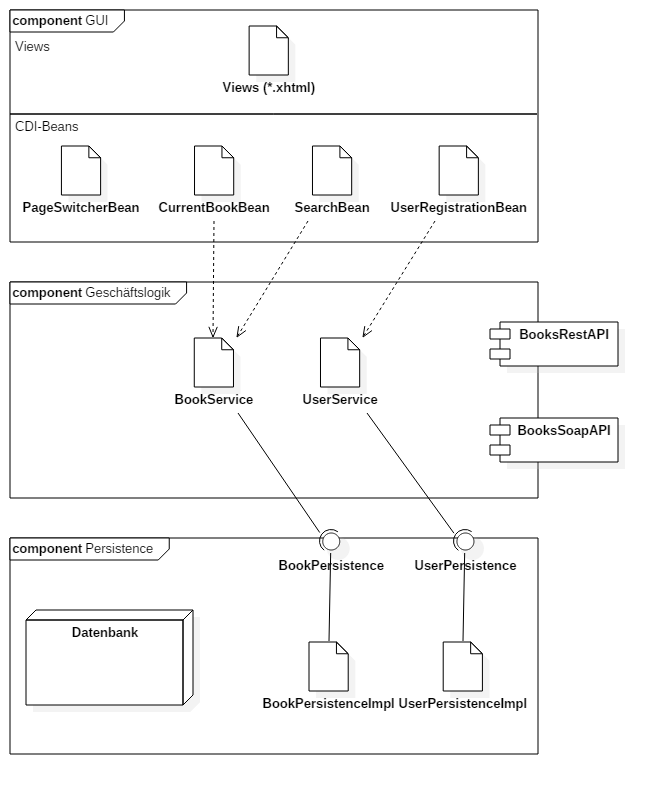
\includegraphics[width=0.70\textwidth]{Images/ComponentDiagram.png}
			\label{componentDiagramm}			
			\caption[Darstellung der Komponenten]{Darstellung der Komponenten}		
		\end{figure}
		\let\cleardoublepage\clearpage	
		\chapter{Package-Struktur}
		Die folgende Abbildung \ref{packageStructur} zeigt die Struktur der Packages der Anwendung.
		\vspace{1cm}		
		\begin{figure}[ht]
			\centering
			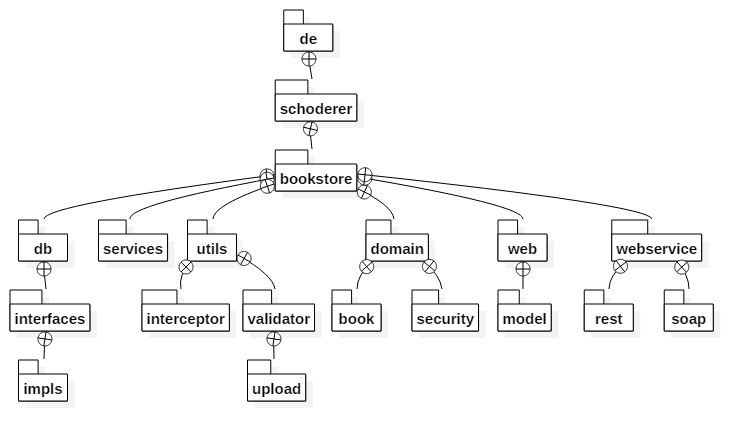
\includegraphics[width=1\textwidth]{Images/package.png}
			\label{packageStructur}			
			\caption[Packetstrukturdiagramm]{Darstellung der Packetstruktur der Anwendung}		
		\end{figure}\\
		
	\underline{\textbf{Beschreibung der Packages}}
		\begin{description}
			\item[bookstore] \hfill \\
			 Dies ist das Hauptpackage der Anwendung
			 	\item[db.interfaces] \hfill \\
				 	Hier liegen die Interfaces, welche die Datenbankzugriffe abkapseln
			 		\item[db.interfaces.impls] \hfill \\
			 		Hier liegen die Implementierungen der Datenbankzugriffsinterfaces
			 	\item[services] \hfill \\
			 	In diesem Package befinden sich die Service-Klassen, welche die Geschäftslogik der Anwendung beinhalten
			\item[utils.validator] \hfill \\
		In diesem Package und dem Unterpacket $upload$ befinden sich die JSF-spezifischen Validatoren, welche die Eingaben der Benutzer validieren
		\item[domain.book] \hfill \\
		Hier befinden sich die Domänenobjekte, welche für den Betrieb der Anwendung benötigt werden 
		\item[domain.security] \hfill \\
		Hier befinden sich die Domänenobjekte, welche die Benutzer und deren Rechte repräsentieren
		\item[web.model] \hfill \\
		In diesem Packet befinden sich die CDI-Beans
		\item[webservice.rest] \hfill \\
		Hier befinden sich die Klassen, welche benötigt werden um die REST-API der Anwendung bereitzustellen
		\item[webservice.soap] \hfill \\
		Hier befinden sich die Klassen, welche benötigt werden um die SOAP-API der Anwendung bereitzustellen
		\end{description}
		
		\chapter{Datenbank}
		\vspace{1cm}
		
		\begin{figure}[ht]
			\centering
			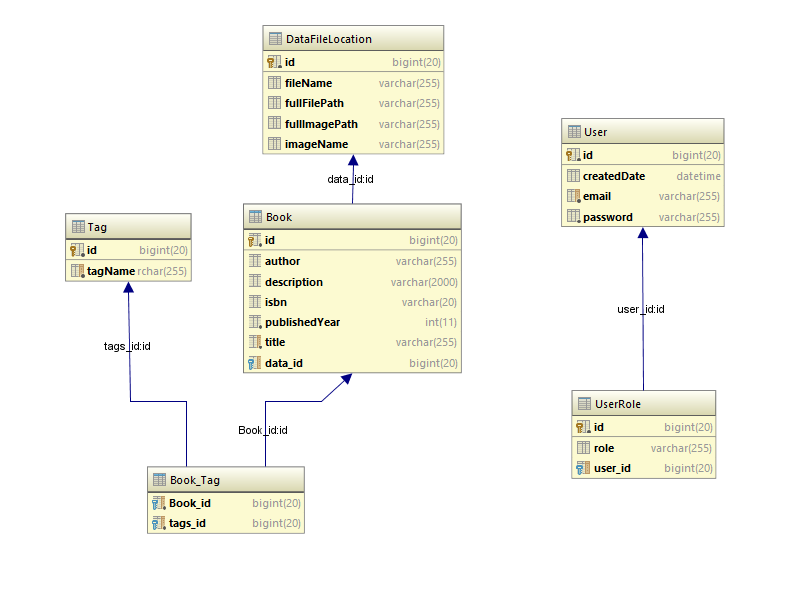
\includegraphics[width=0.8\textwidth]{Images/database.png}
			\caption[Datenbankdiagram]{Modell der Datenbank der Anwendung}
			\label{database}
		\end{figure}
		
		\begin{description}
			\item[\underline{$Book$}] \hfill \\
				In der Tabelle $Book$  werden alle Informationen zu einem Buch gespeichert
			\item[\underline{$DataFileLocation$}] \hfill \\
			In der Tabelle $DataFileLocation$  wird der Speicherort der Dateien auf dem Filesystem festgehalten, sowie der Name der Dateien. Die Tabelle DataFileLocation steht in einer 1-zu-1-Beziehung mit der Tabelle $Book$
			\item[\underline{$Tag$}]\hfill \\
				In dieser Tabelle werden die Tags zu den Büchern gespeichert. Zwischen der Tabelle Tags und der Tabelle $Book$ besteht eine n-zu-m-Beziehung, weshalb die Zuordnung der Tags zu den Büchern über die Tabelle $Book\_Tag$ verwaltet wird
				\item[\underline{$Book\_Tag$}]\hfill \\
				Diese Tabelle ist eine Mapping-Tabelle zwischen $Book$ und $Tag$
				\item[\underline{$User$}]\hfill \\
				In dieser Tabelle werden die Daten der registrierten Benutzer der Anwendung gespeichert
				\item[\underline{$UserRole$}]\hfill \\
				Die $UserRole$-Tabelle ordnet jedem Benutzer in der $User$-Tabelle eine oder mehrere Rollen zu
		\end{description}
		\chapter{Webservices}
		Die beiden Webservices der Anwendung erlauben Zugriff auf die CRUD-Methoden zum Erstellen, Bearbeiten, Lesen und Löschen eines Buches. Die Webservices greifen direkt auf die Klasse $BookService$ der Geschäftslogik zu.
		\section{REST-API}
		Die REST-API ist unter \href{http://mschoderer.de:8080/bookstore/api/rest/books}{http://mschoderer.de:8080/bookstore/api/rest/books} erreichbar und bietet über die für REST typischen HTTP-Methoden (GET, POST, PUT, DELETE) zugriff auf die Anwendung. Für die Serialisierung der Objekte verwendet die Schnittstelle das JSON-Format.
		\section{SOAP-API}
		Die wsdl-File für die SOAP-API kann unter \href{http://mschoderer.de:8080/bookstore/BooksSoapApi?wsdl}{http://mschoderer.de:8080/bookstore/BooksSoapApi?wsdl} erhalten werden.
		
		
\end{document}